% lab02

\section{Lab 2}

All the following analysis are extrapolated from a visual inspection of the
histograms and scatterplots, therefore they aren't quantitative and misurable
evaluations, but just qualitative findings evaluated by eye.
The first two features are unimodal, but they overlap too much and we can say
that they could not be useful in the discrimination of the two classes (PCA? Variance?)
The last two, are slightly overlapped, but multimodal so we can say that a simple linear
model could not be sufficient to well discriminate the two classes among data.
The third and the fourth features instead are unimodal and don't overlap so much,
so probably they are the most useful traits in the data we have. In an LDA analysis,
probably the first components would be a linear combination of the features that
highly correspond to the direction of the third and the fourth features, since LDA
tend to select linear combination of the features in a way that the first component
is the more "discriminant", in the sense that classes are highly distinguishable.
PCA? (variance almost the same among features, already normalized data?)

\begin{figure}[htbp]
    \centering
    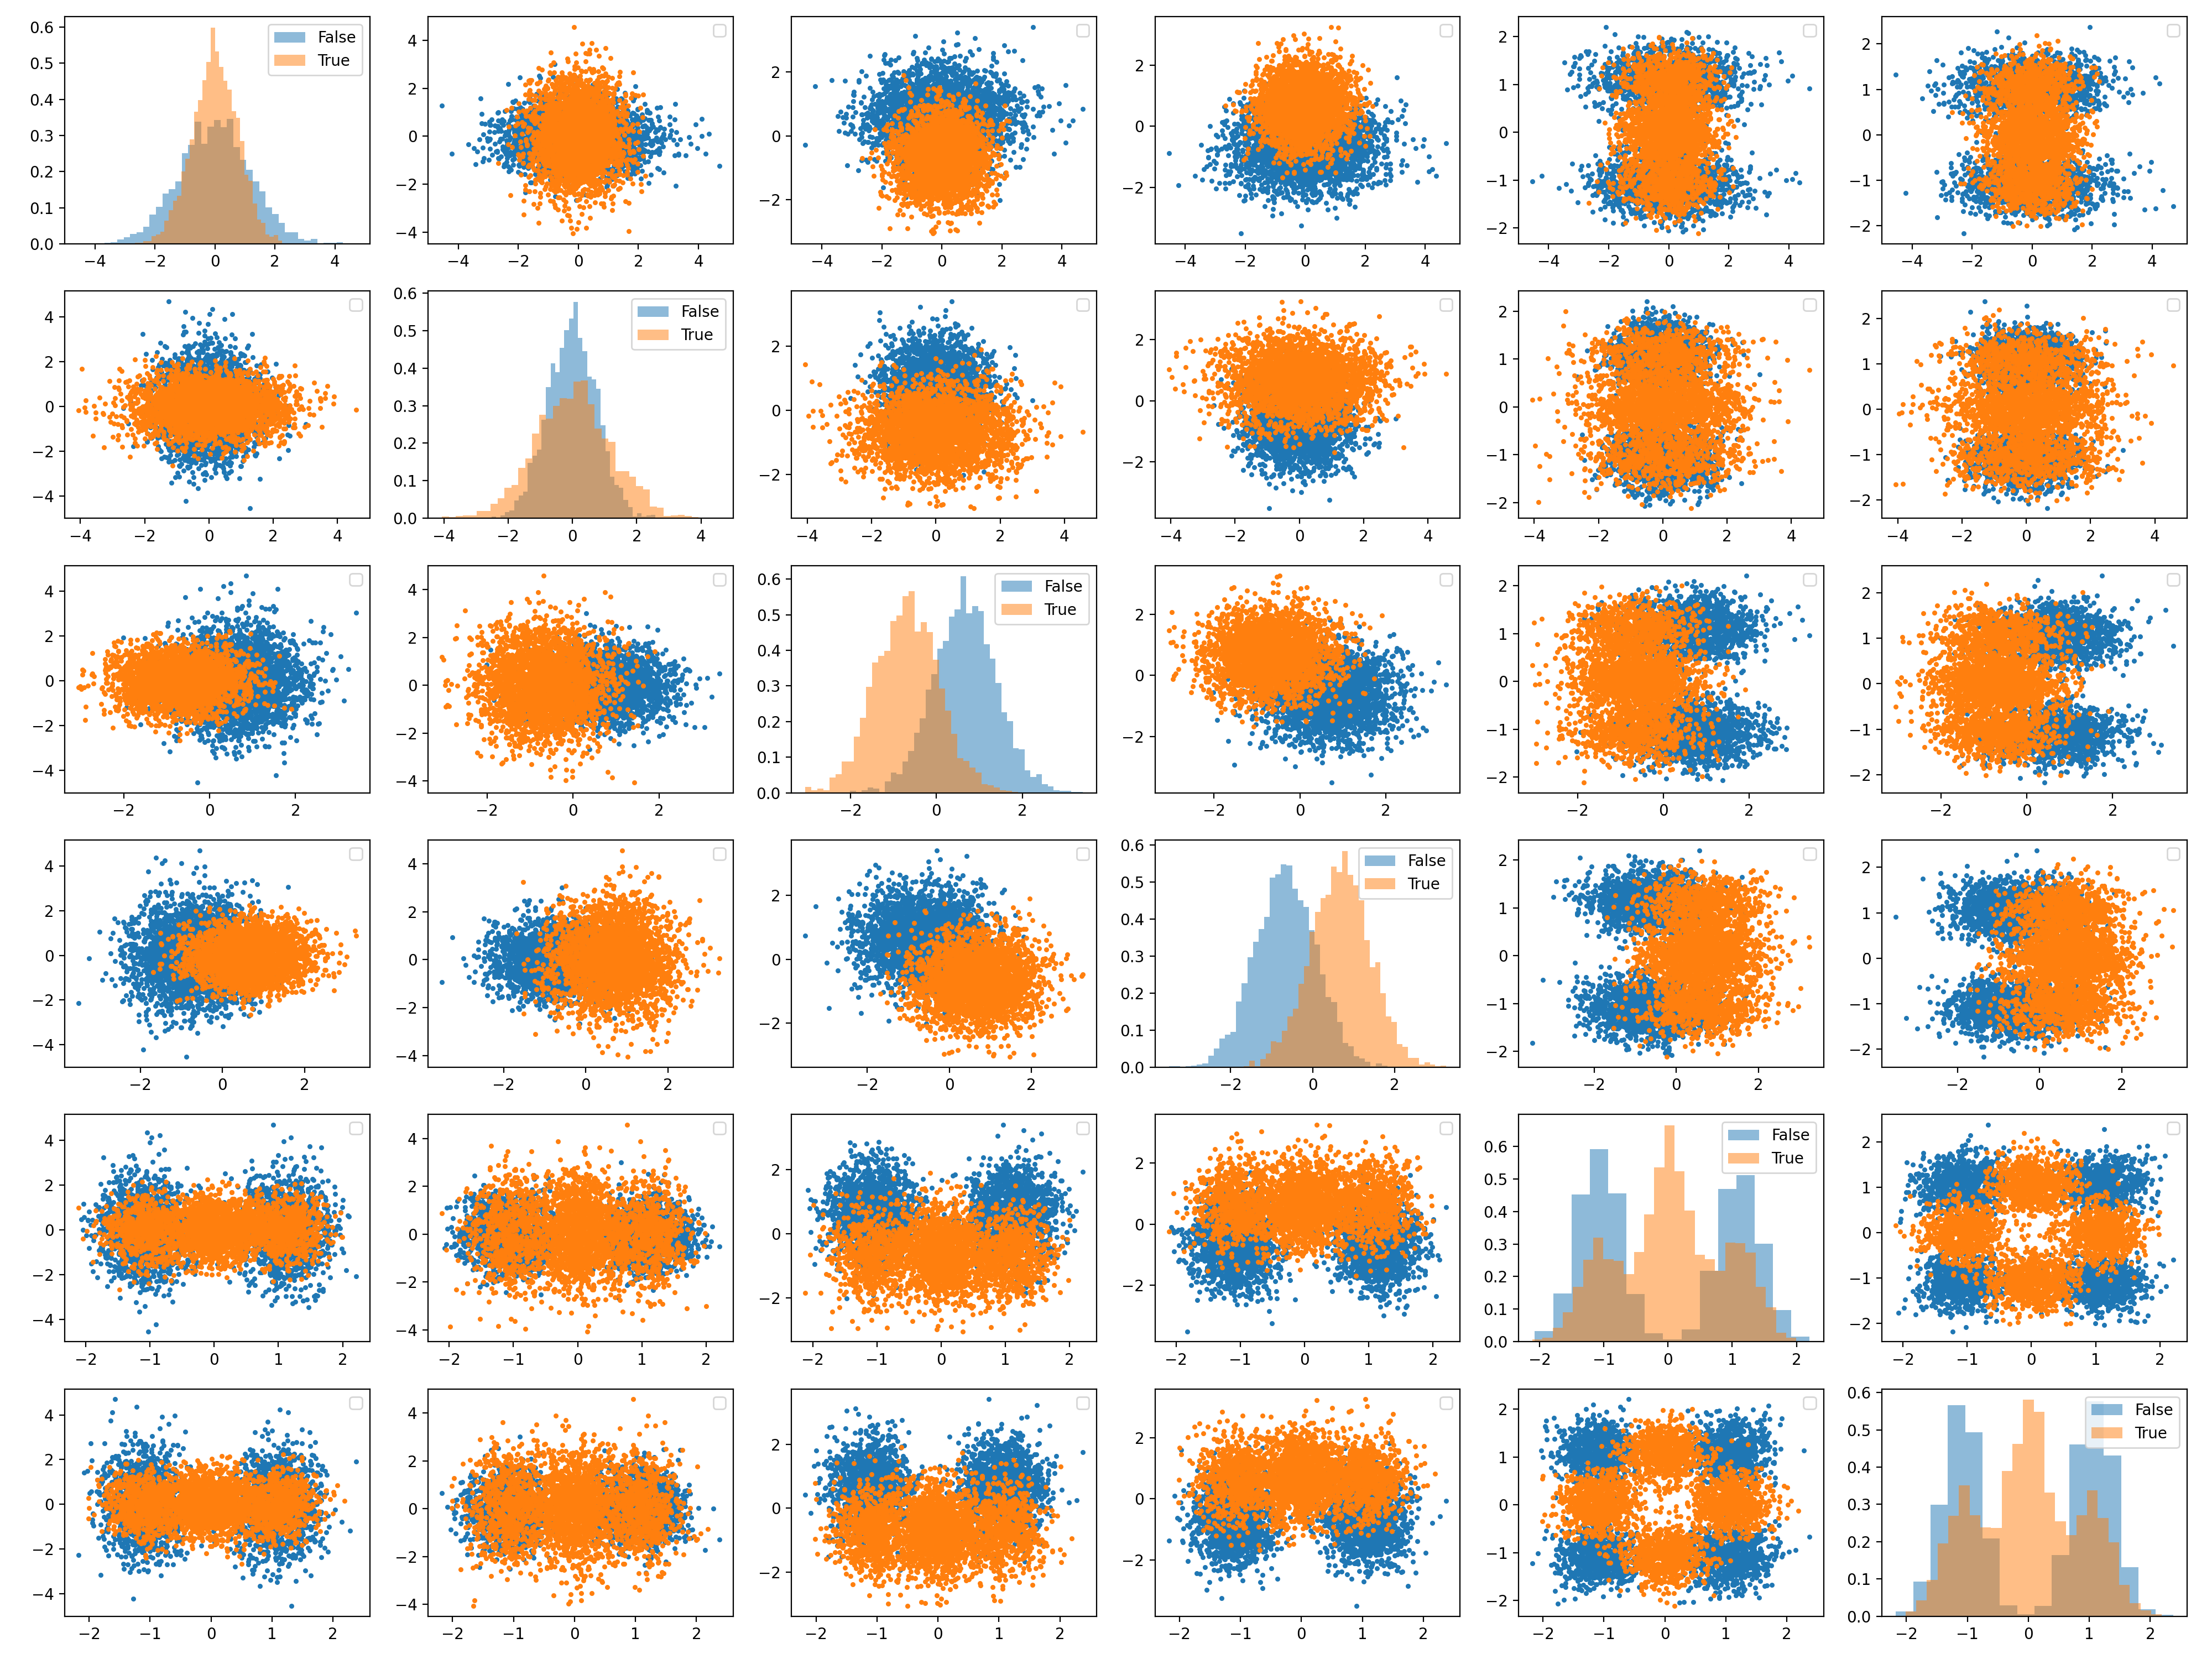
\includegraphics[width=0.9\linewidth]{lab02/scatter.png} % Adjust the width as needed
    \caption{Spoofing dataset scatter and histogram plots}
    \label{fig:scatter}
\end{figure}